% arara: xelatex
% arara: xelatex
% arara: xelatex


% options:
% thesis=B bachelor's thesis
% thesis=M master's thesis
% czech thesis in Czech language
% english thesis in English language
% hidelinks remove colour boxes around hyperlinks

\documentclass[thesis=B,english]{FITthesis}[2019/03/21]

\usepackage{todonotes}

%\usepackage[utf8]{inputenc} % LaTeX source encoded as UTF-8
% \usepackage[latin2]{inputenc} % LaTeX source encoded as ISO-8859-2
% \usepackage[cp1250]{inputenc} % LaTeX source encoded as Windows-1250

% \usepackage{subfig} %subfigures
% \usepackage{amsmath} %advanced maths
% \usepackage{amssymb} %additional math symbols

\usepackage{dirtree} %directory tree visualisation

% % list of acronyms
% \usepackage[acronym,nonumberlist,toc,numberedsection=autolabel]{glossaries}
% \iflanguage{czech}{\renewcommand*{\acronymname}{Seznam pou{\v z}it{\' y}ch zkratek}}{}
% \makeglossaries

% % % % % % % % % % % % % % % % % % % % % % % % % % % % % % 
% EDIT THIS
% % % % % % % % % % % % % % % % % % % % % % % % % % % % % % 

\department{Department of Software Engineering}
\title{Thesis title (SPECIFY)}
\authorGN{Zuzana} %author's given name/names
\authorFN{Václaviková} %author's surname
\author{Zuzana Václaviková} %author's name without academic degrees
\authorWithDegrees{Zuzana Václaviková} %author's name with academic degrees
\supervisor{Ing. Jan Krákora, PhD.}
\acknowledgements{THANKS (remove entirely in case you do not with to thank anyone)}
\abstractEN{Summarize the contents and contribution of your work in a few sentences in English language.}
\abstractCS{V n{\v e}kolika v{\v e}t{\' a}ch shr{\v n}te obsah a p{\v r}{\' i}nos t{\' e}to pr{\' a}ce v {\v c}esk{\' e}m jazyce.}
\placeForDeclarationOfAuthenticity{Prague}
\keywordsCS{Internet věcí, nositelná elektronika, turistika, tělesná kondice}
\keywordsEN{Internet of Things, smart wearables, hiking, fitness}
\declarationOfAuthenticityOption{1} %select as appropriate, according to the desired license (integer 1-6)
% \website{http://site.example/thesis} %optional thesis URL


\begin{document}

% \newacronym{CVUT}{{\v C}VUT}{{\v C}esk{\' e} vysok{\' e} u{\v c}en{\' i} technick{\' e} v Praze}
% \newacronym{FIT}{FIT}{Fakulta informa{\v c}n{\' i}ch technologi{\' i}}

REMOVE THIS
\linebreak
Analysis of an IoT solution for assessment of tourist track physical difficulty

The aim of this thesis is to analyse, design and implement a proof-of-concept \todo{maybe change the way the acronyms are introduced?} (PoC) Internet-of-Things (IoT) solution for tourist track difficulty estimation.
Using a mobile application, the user shall be able to select a track and assess how difficult the specific part of the track will be for them, based on data collected from similarly fit users.
\begin{itemize}
    \item Analyse and compare similar existing solutions.
    \item Analyse and design an IoT solution for data processing.
    \item Design a mobile application for data visualization and track selection.
    \item Create a PoC of the IoT platform and of the mobile application.
    \item Collect raw data from smart watch heart rate sensors and smart phone GPS locators and propose relevant statistics to process this data.
\end{itemize}


\setsecnumdepth{part}
\chapter{Dictionary}
\begin{description}
	\item[IoT] Internet of Things -- \textit{The interconnection via the Internet of computing devices embedded in everyday objects, enabling them to send and receive data} \cite{IoT-dictionary} without requiring human-to-human or human-to-computer interaction. \cite{IoT-definition-no-interaction}
	\item[PoC] Proof of Concept -- \textit{Evidence, typically deriving from an experiment or pilot project, which demonstrates that a design concept, business proposal, etc. is feasible.} \cite{PoC-dictionary}
\end{description}

\chapter{Introduction}
With the increasing popularity of smart wearables in the general public, a growing number of people have been able to benefit from adjustments in their behaviour according to the way their data gets processed and fed back to them.
Runners can barely imagine not checking how fast and how efficiently they just ran their daily track or how much they have improved over the last month,
people with sedentary jobs attempt to keep their daily step count above a currently recommended number,
masses of people have been saving up for the Apple Watch 5~\cite{AppleWatch5} in spite of the ECG health monitor being virtually unnecessary for those not at risk of cardiac disease~\cite{ecg-screening}, etc.

All of this data is collected from a variety of devices, such as smartwatches, textiles with integrated sensors, jewelry, or more invasive ones such as implants or tattoos, all of which are meant to be worn on the user's body and which measure and send data for analysis - hence the name \textit{wearable technology}, or \textit{smartwear}~\cite{what-is-wearable-tech}.

Thanks to the data collected from these devices, the users have been keeping track of their health and fitness, setting goals for themselves and tracking personal achievements.
However, all of this is related to the past of each individual user, while the true potential of smartwear lies in collecting data from thousands of people,
finding patterns and correlations in large datasets and using the results to increase precision and improve upon whatever the data is being used for by the virtue of prediction.

That being said, the result of this thesis will be a design for an IoT solution, mainly to be used by hikers who want to not only pick a track on a map and see how long it is going to take them to get from point A to point B (which generally isn't tailored to the individual's fitness and often doesn't account for the possible rapid changes in the track's elevation profile),
but also an objective difficulty level of particular sections of said track, which may have additional benefits for people with cardiac issues or those trying to lose weight, who are interested in some more detailed insight into the exertion induced by the track in order to keep their heart rate in a specific range.
All of this will be available to the user before stepping foot on said track, thanks to the data collected from users with various fitness levels and their own history,
while the user's fitness will be presented more accurately as they continue to use the application.

I will study how fitness is assessed in regard to feasibility, availability for the general public, and precision, in order to provide fundamentals for further work.

Using methods of software engineering, I am going to analyse the use of wearable technology in existing applications and document the most common features as well as their outstanding traits and their use of IoT principles (or lack thereof).
Based on this analysis, I will pick the most relevant features to include in my design and extend them with features of my own devising, which will set my solution apart from existing software.

I will design and implement a PoC IoT solution -- a mobile application which will collect data from the smartwear sensor and an available GPS locator, along with a backend IoT platform to receive and process collected data, and the communication channels used between these two modules.
I will neither design nor implement a full-fledged IoT platform as that's not in the scope of this thesis.
I will design (not implement) the frontend mobile application for displaying of processed data, track selection with integrated maps and explore the necessary legal requirements for the use of such maps.

I will examine the use of different device types with heart rate sensors and choose one with which I will build my PoC.

I will collect and perform suitable operations on the collected data in order to visualize it.



\setsecnumdepth{all}
\chapter{Existing solutions}
There's a plethora of applications taking advantage of wearable tech, not all of them using the available bio sensors, ranging from basic real-time heart rate monitoring to progress tracking, to calorie measuring, and to social network sized fitness communities.

In this chapter I will research a few such applications, compare and rate them based on following criteria. \todo{add weight to individual points}
\begin{itemize}
    \item Use of IoT possibilities -- use of available sensors, data collection from the community,
    \item User fitness assessment -- how the user's fitness is assessed (attempt self-assessment, fill out a questionnaire, or take a physical test),
    \item Track difficulty assessment -- how the track's difficulty is assessed (user-reported, or calculated)
    \item Community -- built-in sharing options, possibility for interaction between users,
    \item Extra features -- interesting perks outside of the scope of my app,
    \item User-friendliness -- navigation around the mobile application - finding the general settings, creating and clearing a route, general user experience,
    \item Availability -- is the application or its parts free, paid or are there microtransactions,
    \item Cross-platform -- major operating systems supporting the mobile application and sensors, if any are used,
    \item Propriety -- whether the solution is open-source, closed-source or else.
\end{itemize}


\subsection{komoot}
The cross-platform application for outdoor track suggestion can also be used as a tour planner, a map and a navigation system.

\todo[color = green]{add numeric ratings}

\subsubsection*{Use of IoT possibilities}
Given its use of GPS sensors, komoot does qualify as a basic IoT system, however, it also relies heavily on user input for track rating.
The smart watch only gets used for displaying of routes and navigation, not taking any advantage of the available sensors.
\subsubsection*{User fitness assessment}
When a user is creating a route, they can set its difficulty as one of five levels, 
describing the user's self-reported physical fitness and their current taste for a challenge (or lack thereof): Couch Potato, Average, In Good Shape, Athletic, and Pro.
This parameter is considered when the app is generating a suitable route -- presumably by trying to adjust the elevation profile of the possible routes.
The user's real fitness is not taken into account.
\subsubsection*{Track difficulty assessment} 
Thanks to the maps provided by the OpenStreetMap, users are able to pick a starting point, a destination, as well as any number of waypoints in between for their route.
Once the route is chosen, the user can go through the route's stats - the estimated time it will take to get from start to finish, its length, the elevation profile (uphill, downhill, highest and lowest points, estimated average speed) and the surfaces and their use in proportion to the route's length.
All this information is delivered in easy-to-understand charts as well as interactive mappings -- using a slider, the user can see which stat applies in which part of the route.

\begin{figure}[h]
    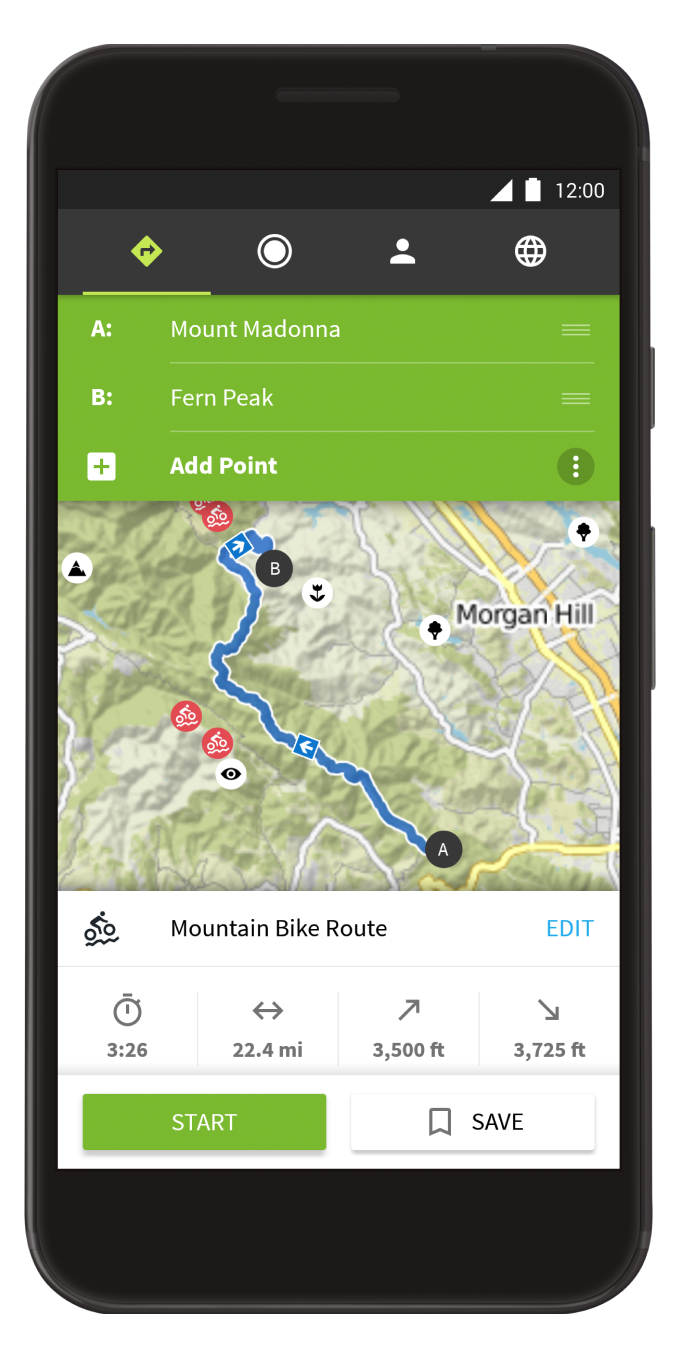
\includegraphics[width=\textwidth]{komoot-nav.png}
    \caption{Offline maps in the komoot app\cite{komoot-nav-img}}
\end{figure}

\begin{figure}[h]
    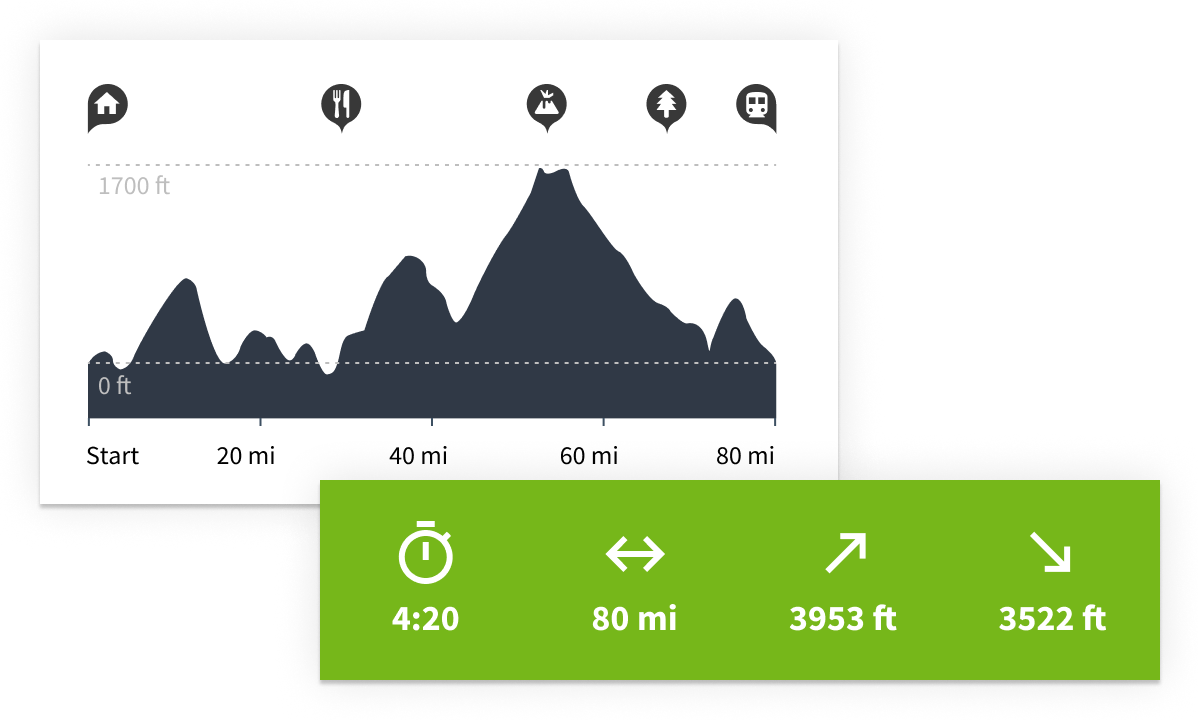
\includegraphics[width=\textwidth]{komoot-route-details.png}
    \caption{Route elevation profile\cite{komoot-route-details-img}}
\end{figure}

\begin{figure}[h]
    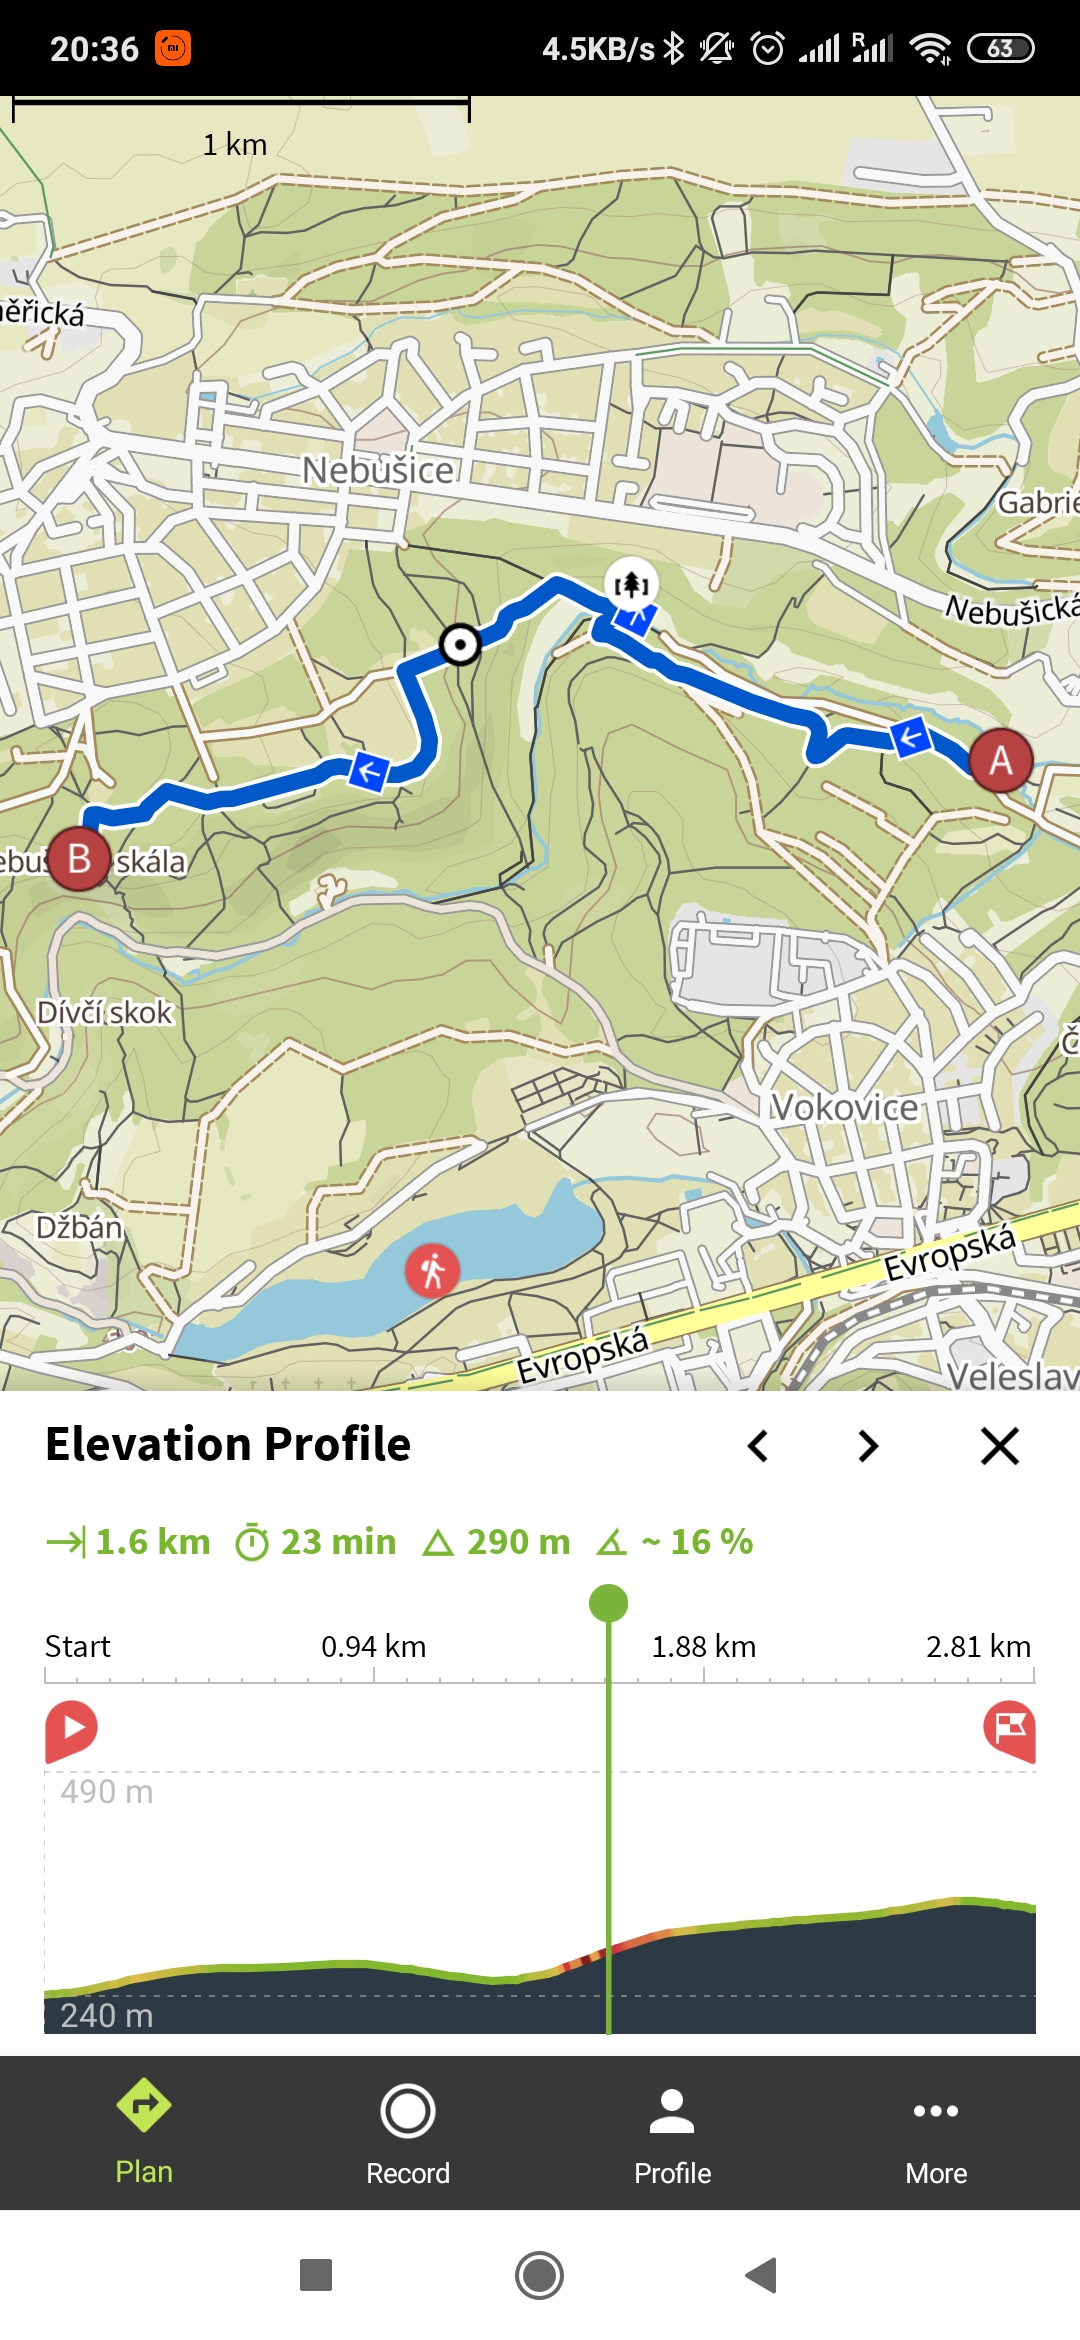
\includegraphics[width=\textwidth]{komoot-route-elevation-detail.jpg}
    \caption{Detailed view of the route's elevation\cite{komoot-route-elevation-detail-img}}
\end{figure}

\begin{figure}[h]
    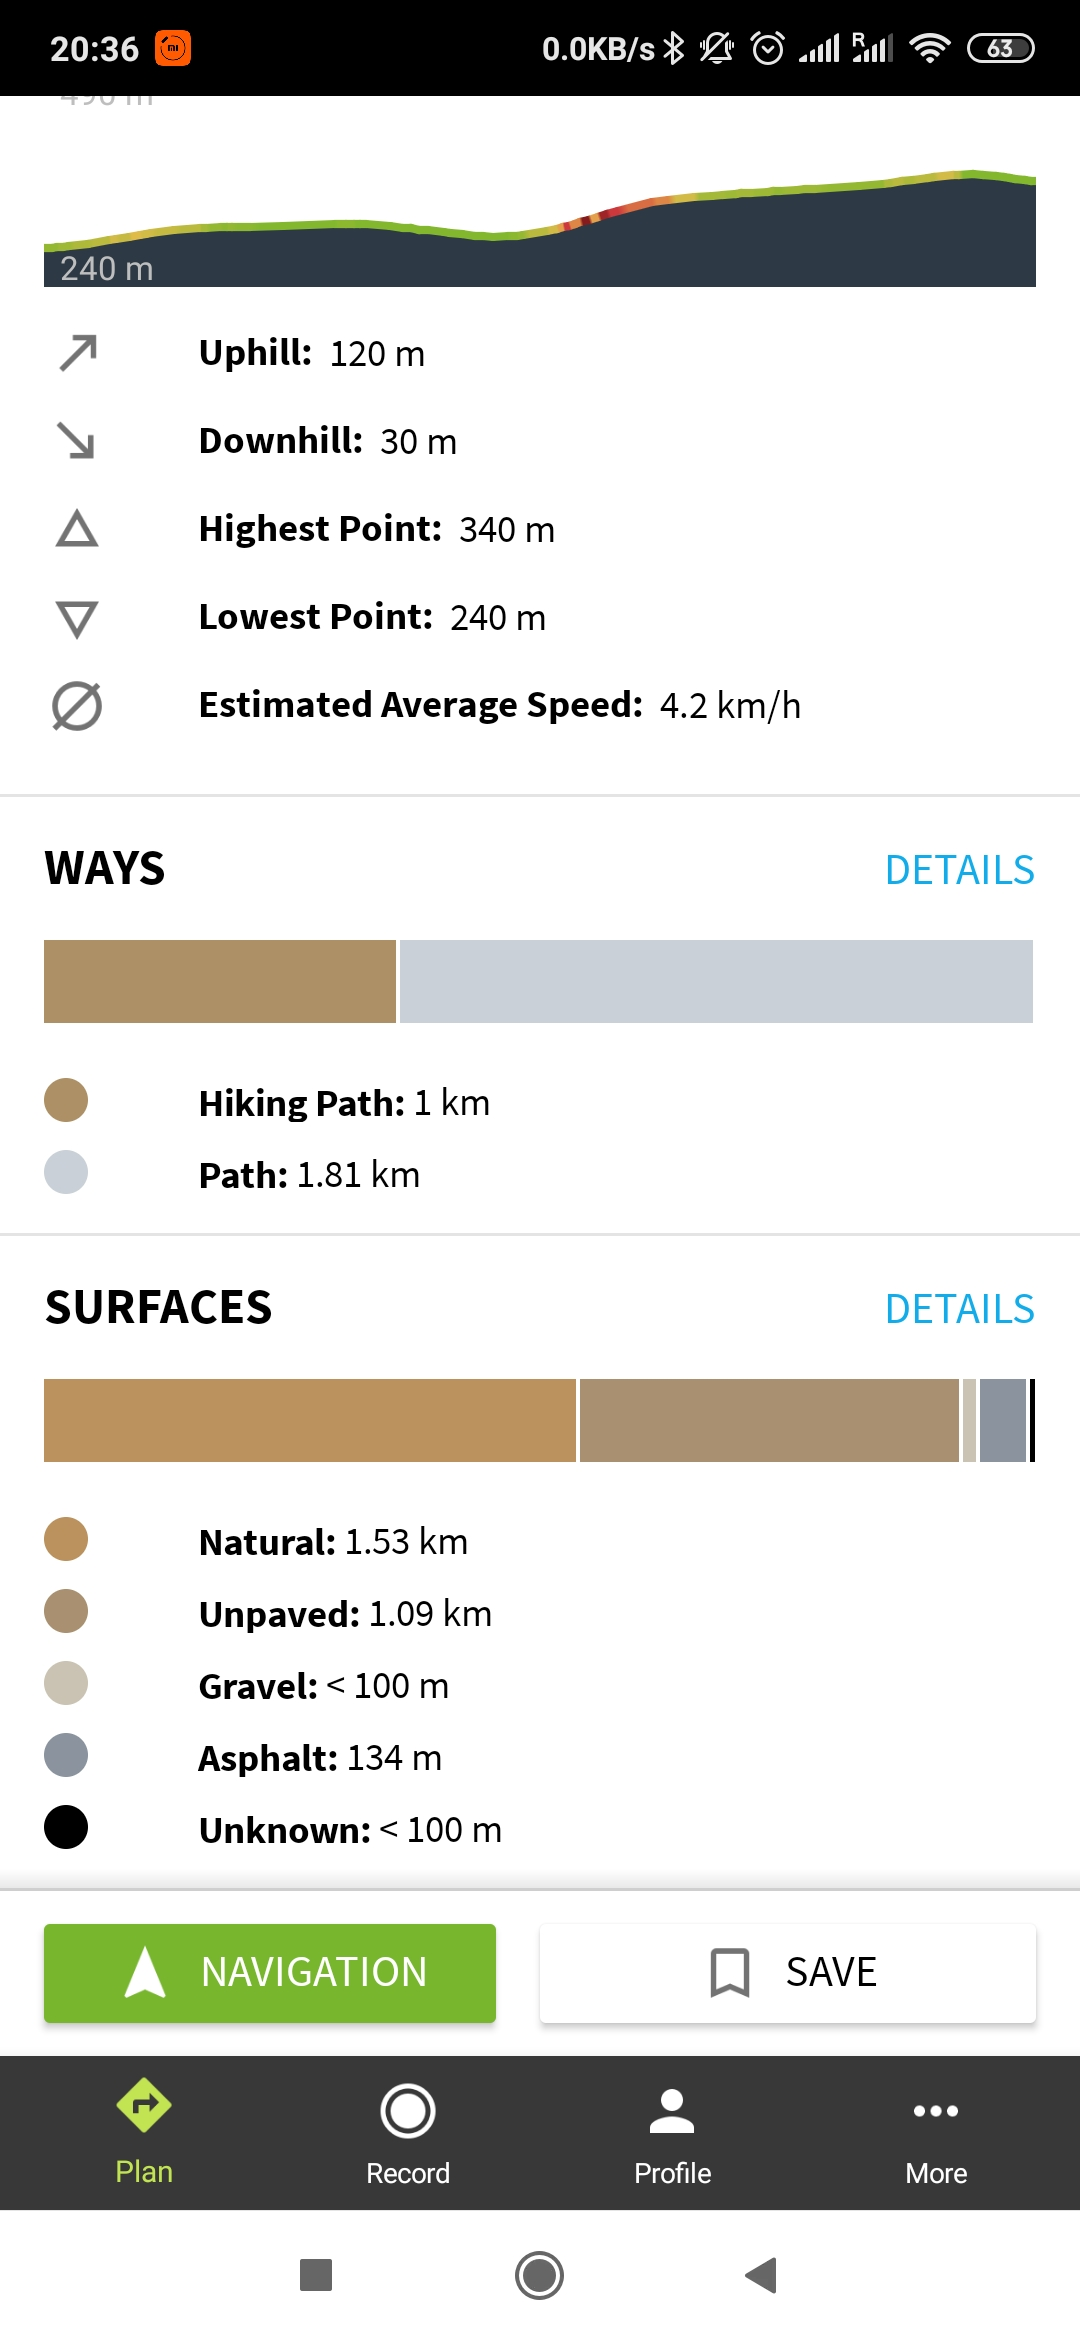
\includegraphics[width=\textwidth]{komoot-route-surface-detail.jpg}
    \caption{Overview of the route's surface. The detailed view is similar to the elevation detail.\cite{komoot-route-surface-overview-img}}
\end{figure}


\subsubsection*{Availability}
The region-based pricing model allows users who do not travel too much to use the app for free,
since the first region is provided at no cost.
In the other pricing options Single Region, Region Bundle and All Regions -- the price-performance ratio seems to grow at a reasonable scale.\todo[color = green]{anything to add?}
\subsubsection*{Community}
With features like sharing of routes users have taken, following of other users, upvoting and commenting on their posts, the mobile application integrates a full-fledged social network.
\subsubsection*{Extra features}

\subsubsection*{User-friendliness}
The navigation through the mobile app takes some time to get used to -- it took me a while to find the Settings after I didn't see them in the burger menu on the bottom navigation bar, which contained only the different pricing options.
Once I created a route, the information provided was well-delivered and easy to read, however, there was no obvious way of completely cancelling the chosen route and picking another one.
Instead, hiding in the Options of the route -- which at first I didn't even notice -- I found the "Reset route" option, which did just what I needed.
Overall, the app has some great parts and some not-so-great ones.
\subsubsection*{Cross-platform}
The system is fully integrated with the Apple Watch and Samsung gear, and -- at least limitedly -- supports a number of other brands of smart watches and other Bluetooth-enabled devices.
The mobile application runs both on iPhones and Android phones.
\subsubsection*{Propriety}
The system is not entirely open-source, as a few of their repositories are public, but the core components remain proprietary. \todo[color = green]{recheck}\todo[color = green]{cite https://github.com/komoot}

\subsubsection*{Overall evaluation}
While being rich with features, komoot doesn't base its functionality on objective data -- it's the users themselves who rate and recommend the specific routes,
an approach in its nature prone to error and with only limited ways of eliminating the human factor.

\subsection{endomondo}
https://www.endomondo.com/
\subsubsection*{Use of IoT possibilities} --
\subsubsection*{User fitness assessment} --
\subsubsection*{Availability} --
\subsubsection*{Community} -- 
\subsubsection*{Extra features} -- 
\subsubsection*{User-friendliness} -- 
\begin{figure}[h]
    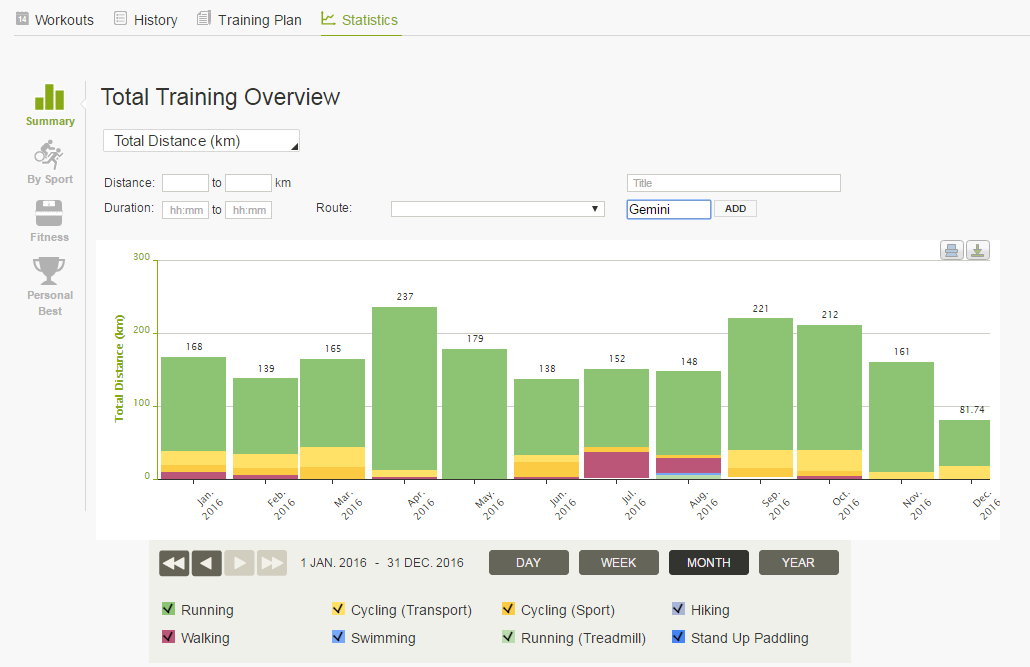
\includegraphics[width=\textwidth]{endomondo-history-example.png}
    \caption{endomondo history example\cite{endomondo-history-img}}
\end{figure}

\begin{figure}[h]
    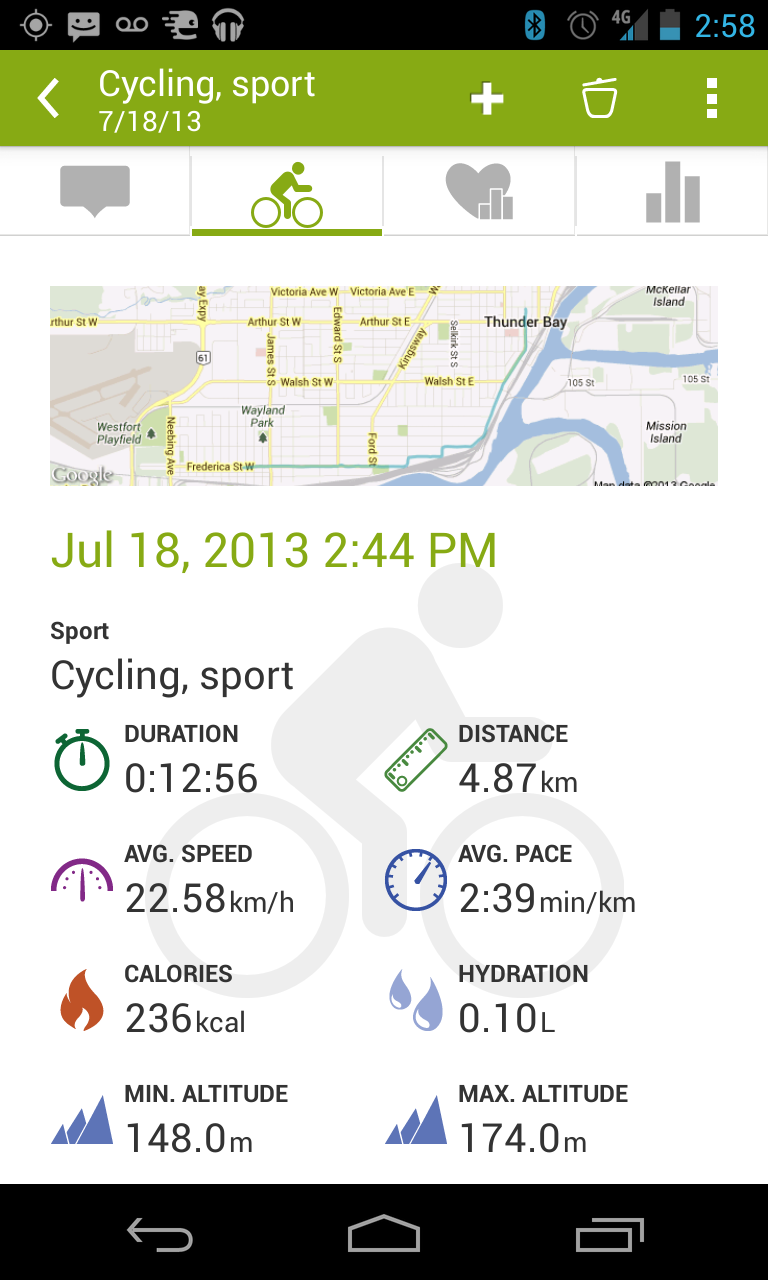
\includegraphics[width=\textwidth]{endomondo-bike-stats.png}
    \caption{Statistics of a biking trip on endomondo\cite{endomondo-bike-stats-img}}
\end{figure}

\subsubsection*{Cross-platform} -- 
\subsubsection*{Propriety} -- 
\subsubsection*{Overall evaluation}

\subsection{Strava}
https://www.strava.com/
\subsubsection*{Use of IoT possibilities} --
\subsubsection*{User fitness assessment} --
\subsubsection*{Availability} --
\subsubsection*{Community} -- 
\subsubsection*{Extra features} -- 
\subsubsection*{User-friendliness}
\begin{figure}[h]
    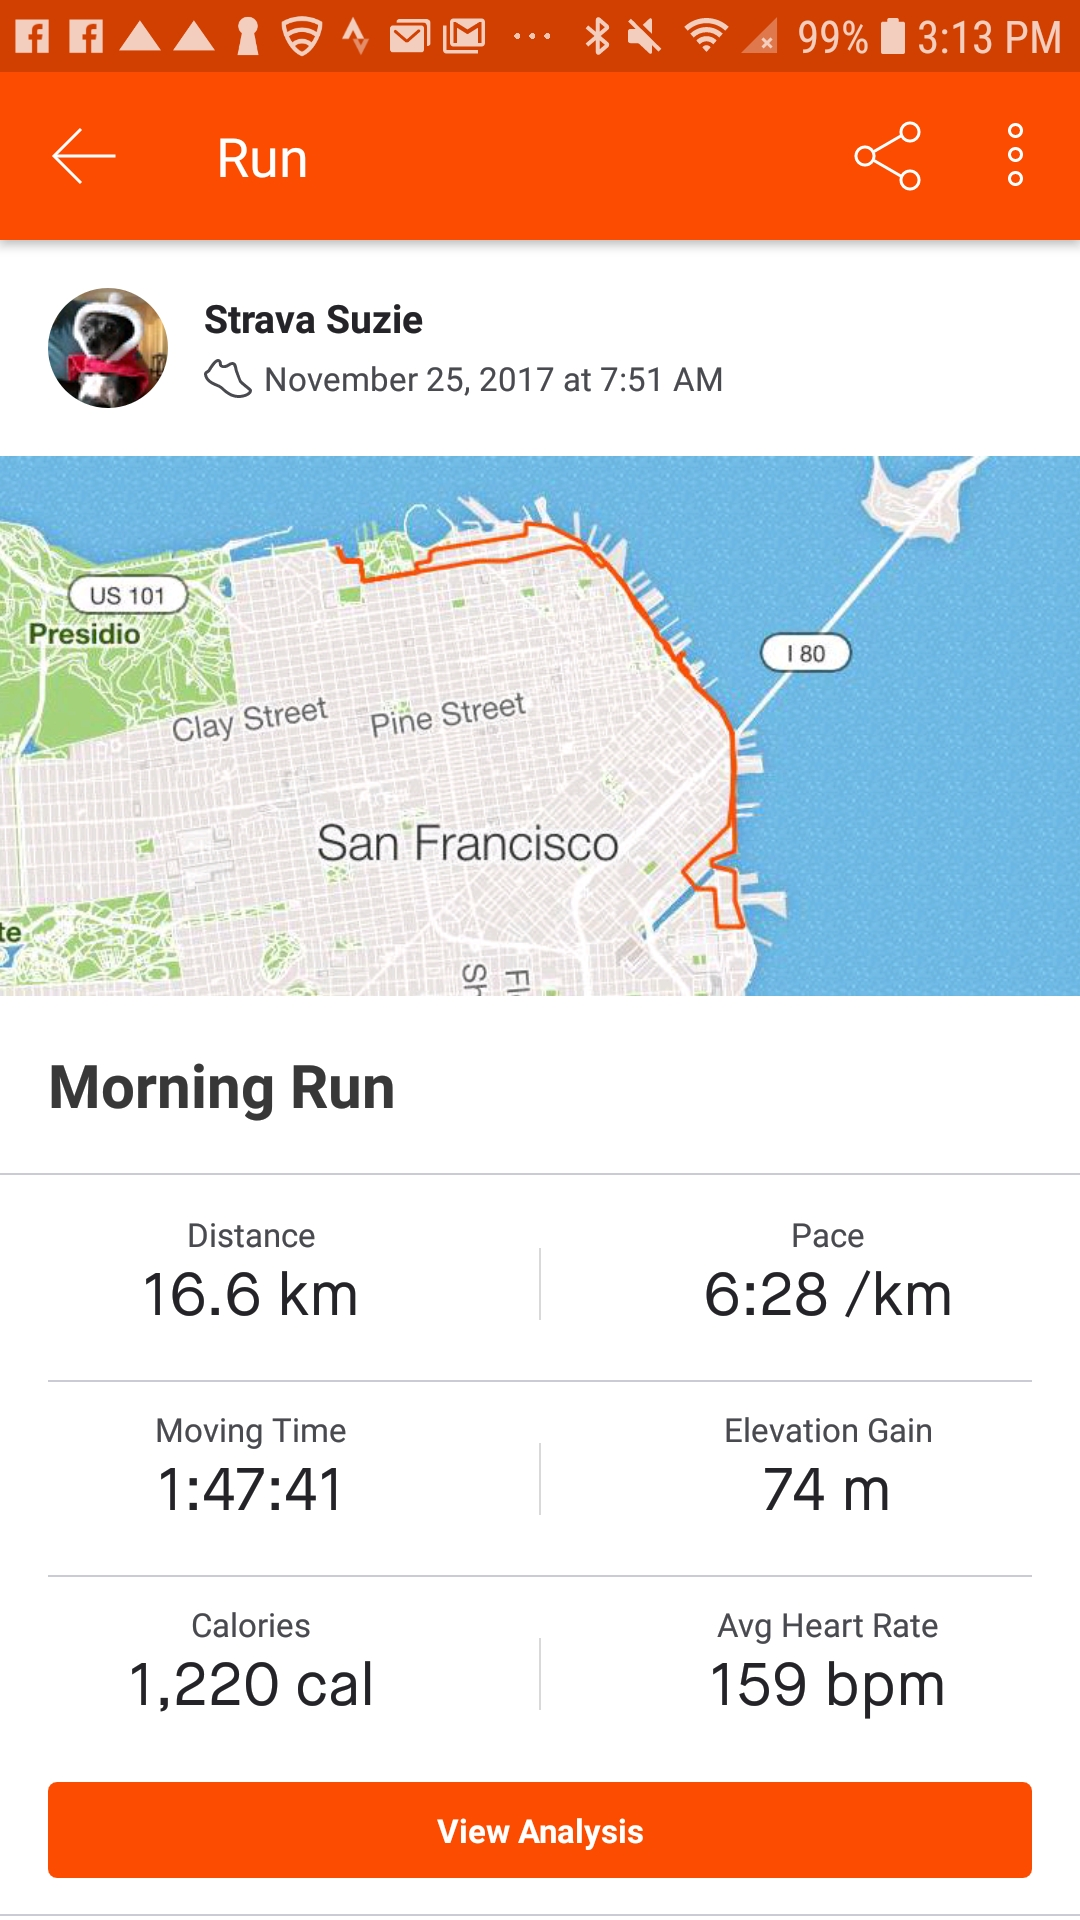
\includegraphics[width=\textwidth]{strava-morning-run-stats.jpg}
    \caption{Statistics of a run on strava\cite{strava-run-stats-img}}
\end{figure}
\subsubsection*{Cross-platform} -- 
\subsubsection*{Propriety} -- 
\subsubsection*{Overall evaluation}

\subsection{myFitnessPal}
https://www.myfitnesspal.com/
\subsubsection*{Use of IoT possibilities} --
\subsubsection*{User fitness assessment} --
\subsubsection*{Availability} --
\subsubsection*{Community} -- 
\subsubsection*{Extra features} -- 
\subsubsection*{User-friendliness} -- 

\begin{figure}[h]
    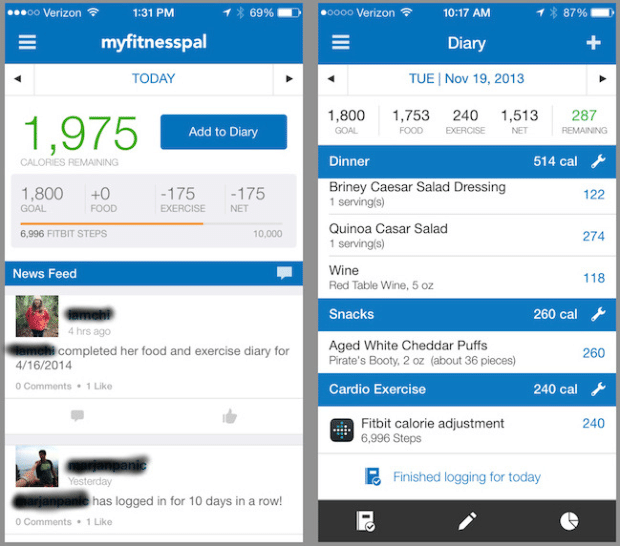
\includegraphics[width=\textwidth]{myfitnesspal-researchgate.png}
    \caption{myFitnessPal feed and diary entry\cite{MFP-diary-img}}
\end{figure}

\subsubsection*{Cross-platform} -- 
\subsubsection*{Propriety} -- 
\subsubsection*{Overall evaluation}

\subsection{Walk with Map My Walk}
https://www.mapmywalk.com/
\subsubsection*{Use of IoT possibilities} --
\subsubsection*{User fitness assessment} --
\subsubsection*{Availability} --
\subsubsection*{Community} -- 
\subsubsection*{Extra features} -- 
\subsubsection*{User-friendliness} -- 

\begin{figure}[h]
    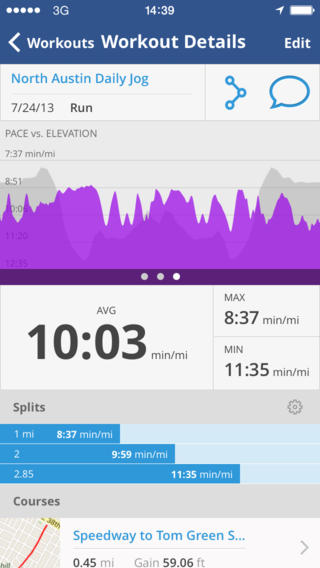
\includegraphics[width=\textwidth]{map-my-fitness-workout-details.jpg}
    \caption{Map my Fitness workout details\cite{map-my-walk-img}}
\end{figure}


\subsubsection*{Cross-platform} -- 
\subsubsection*{Propriety} -- 
\subsubsection*{Overall evaluation}

\subsection{Garmin Explore and Garmin Connect}
The vast ecosystem Garmin has created for their users is filled with an assortment of wearables, radars, smart lights, navigations, customized maps, and plenty more, providing features which are presented to the user via modular mobile apps.

Here I will analyse the Garmin Explore application, which is targeted at hikers, in tandem with Garmin Connect, which functions as a fitness tracker.

\subsubsection*{Use of IoT possibilities}
Most fitness-focused Garmin watches do have a heart rate sensor and all of them include a step counter, however, this data is never compared with that of other users, keeping focus on the user's activity history with no prediction.
\subsubsection*{User fitness assessment}
Some of the heart-rate-monitor enabled watches allow a user to set the zones in which they would like to keep their heart rate depending on the activity they choose to do. The standard zones are:
\textit{
\begin{itemize}
    \item Zone 1 (Warm Up) --
    Perceived exertion: Relaxed, easy pace, rhythmic breathing. Benefits: Beginning-level aerobic training, reduces stress.
    \item Zone 2 (Easy) --
    Perceived exertion: Comfortable pace, slightly deeper breathing, conversation possible. Benefits: Basic cardiovascular training, good recovery pace.
    \item Zone 3 (Aerobic) --
    Perceived exertion: Moderate pace, more difficult to hold conversation. Benefits: Improved aerobic capacity, optimal cardiovascular training.
    \item Zone 4 (Threshold) --
    Perceived exertion: Fast pace and a bit uncomfortable, breathing forceful. Benefits: Improved anaerobic capacity and threshold, improved speed.
    \item Zone 5 (Maximum) --
    Perceived exertion: Sprinting pace, unsustainable for long period of time, labored breathing. Benefits: Anaerobic and muscular endurance, increased power.\cite{garmin-heart-zones}
\end{itemize}
}

\begin{figure}[h]
    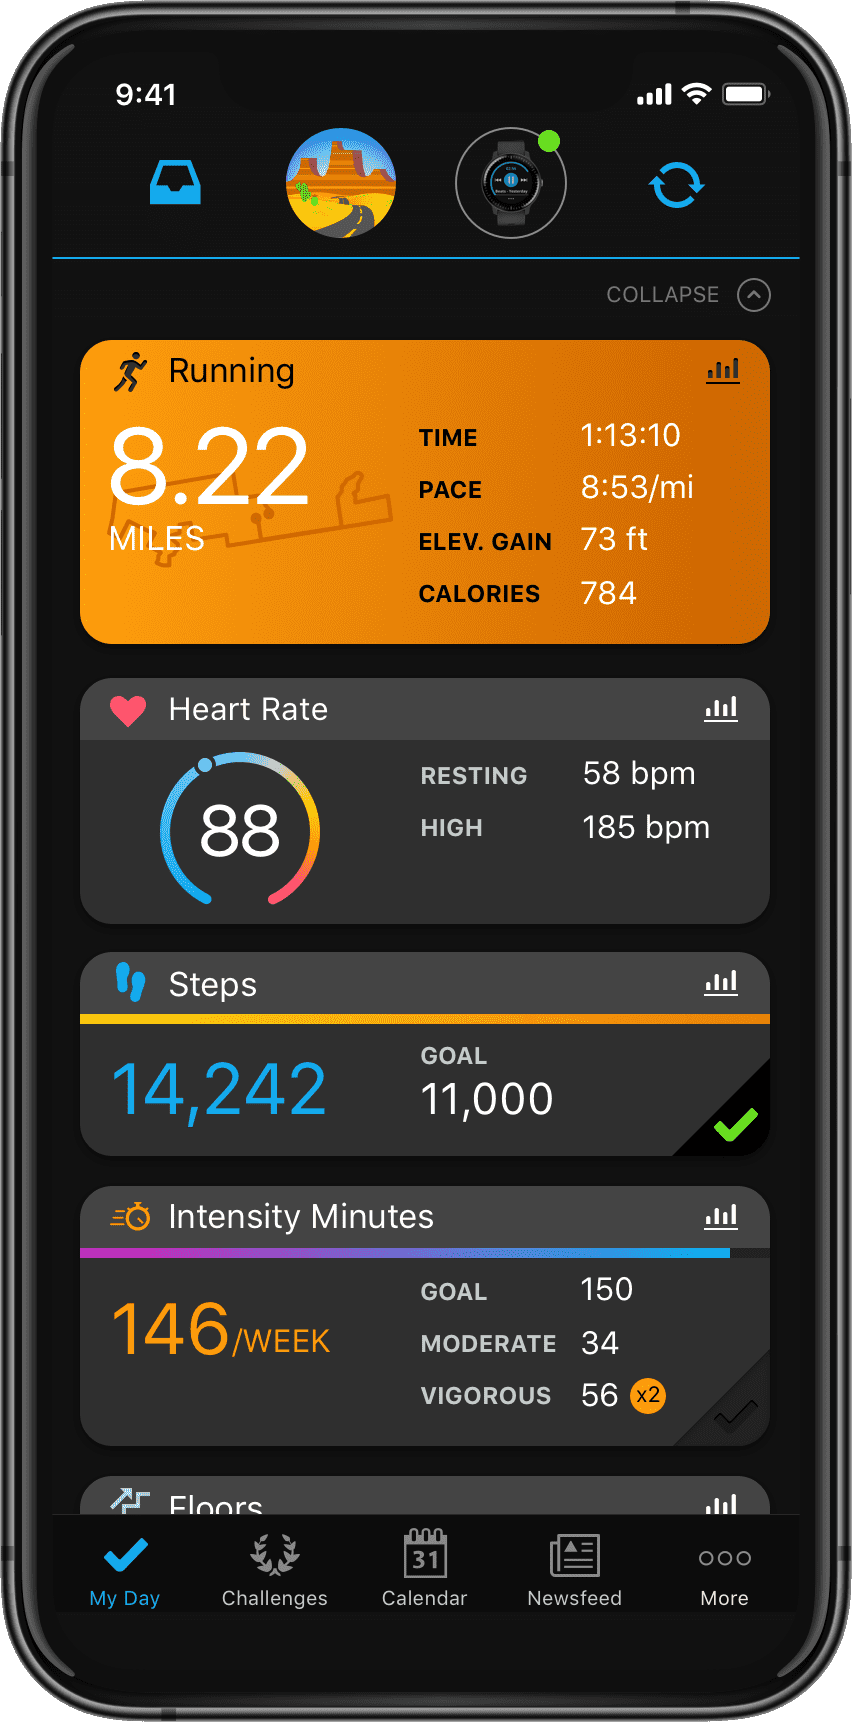
\includegraphics[width=\textwidth]{garmin-connect-myday-screen.png}
    \caption{My day - Garmin Connect's home screen displays statistics of the user's recent activity\cite{garmin-my-day-img}}
\end{figure}

\subsubsection*{Track difficulty assessment}

\subsubsection*{Availability}
In general, Garmin's pricing model relies on the user buying one of their high-end smartwatches, whereupon the rest of the components (apps, basic maps, support, etc.) are free, with some exceptions, such as advanced maps. 
The company's smartwatches are considered premium quality, with a wide price range - target groups include \textit{potential Rolex buyers}\cite{garmin-expensive} as well as ordinary users.\cite{garmin-watches-review}
\subsubsection*{Community}
The Connect application handles the data from the point of view of a fitness tracker, with social features like groups, competitions, likes, comments, and badges of accomplishment.\cite{garmin-connect}
\subsubsection*{Extra features} -- 
\subsubsection*{User-friendliness}

\subsubsection*{Cross-platform}
All of Garmin's applications can be installed both on Android and iPhone.
However, they can only be paired with watches inside Garmin's ecosystem, which is a drawback for users who already own a smartwatch.
\subsubsection*{Propriety}
Some of the Garmin applications are completely open-source, either due to the software that they are derived from, or simply to provide the general public with opportunity to customize their Garmin experience.\cite{garmin-open-source}\cite{garmin-connect-github-repos}
These apps are mostly concerned with map handling, navigation and sound codecs, but also include some bits of functionality like widgets, low power watch apps and others.

While some of this code may be used in the Explore or Connect applications, these repositories don't contain their core functionality.

\subsubsection*{Overall evaluation}
As a fitness tracker, Garmin Connect can definitely be considered acceptable...

\chapter{Analysis and design}

\chapter{Realisation}

\setsecnumdepth{part}
\chapter{Conclusion}


\bibliographystyle{iso690}
\bibliography{mybibliographyfile}

\setsecnumdepth{all}
\appendix

\chapter{Acronyms}
% \printglossaries
\begin{description}
	\item[GUI] Graphical user interface
	\item[XML] Extensible markup language
\end{description}


\chapter{Contents of enclosed CD}

%change appropriately

\begin{figure}
	\dirtree{%
		.1 readme.txt\DTcomment{the file with CD contents description}.
		.1 exe\DTcomment{the directory with executables}.
		.1 src\DTcomment{the directory of source codes}.
		.2 wbdcm\DTcomment{implementation sources}.
		.2 thesis\DTcomment{the directory of \LaTeX{} source codes of the thesis}.
		.1 text\DTcomment{the thesis text directory}.
		.2 thesis.pdf\DTcomment{the thesis text in PDF format}.
		.2 thesis.ps\DTcomment{the thesis text in PS format}.
	}
\end{figure}

\end{document}
